%======================================================================
% T8_Phase_transitions.pdf
%======================================================================
\section{Cvičení: Fázové přechody}
\strana{T8-1}

\begin{priklad}[Příklad 1]
Najděte kritický bod vdW izotermy $(T_c, v_c, p_c)$ a vyjádřete stavovou rovnici a hustotu volné energie $f(T,v)$
v redukovaných proměnných $\tau = T/T_c$, $\nu = v/v_c$ \& $\tilde p = p/p_c$.
\end{priklad}

\begin{priklad}[Příklad 2]
Ukažte, že Gibbsův potenciál z příkladu z přednášky
\begin{center}
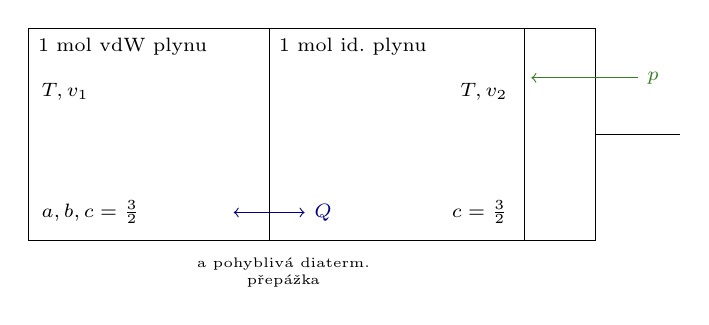
\begin{tikzpicture}[scale=0.9]
  \draw (0,0) rectangle (3.4,3);
  \draw (3.4,0) rectangle (7,3);
  \draw (7,0) -- (8,0) -- (8,3) -- (7,3);
  \draw (8,1.5) -- (9.2,1.5);
  \node[anchor=north west,font=\scriptsize] at (0,3) {1 mol vdW plynu};
  \node[anchor=north west,font=\scriptsize] at (3.4,3) {1 mol id.\ plynu};
  \node[anchor=west,font=\scriptsize] at (0.05,2.1) {$T, v_1$};
  \node[anchor=east,font=\scriptsize] at (6.9,2.1) {$T, v_2$};
  \node[anchor=west,font=\scriptsize] at (0.05,0.4) {$a, b, c = \frac32$};
  \node[anchor=east,font=\scriptsize] at (6.9,0.4) {$c = \frac32$};
  \draw[<->,NavyBlue] (2.9,0.4) -- (3.9,0.4) node[right,font=\scriptsize] {$Q$};
  \draw[<-,OliveGreen] (7.1,2.3) -- (8.6,2.3) node[right,font=\scriptsize] {$p$};
  \node[font=\tiny,align=center] at (3.6,-0.45) {a pohyblivá diaterm.\\ přepážka};
\end{tikzpicture}
\end{center}
lze napsat ve tvaru
\[
  g(\tau,\tilde p,\nu_1) = \frac{a}{9b}\,\tilde g(\tau,\tilde p,\nu_1)
\]
\[
  \tilde g(\tau,\tilde p,\nu_1) = \frac{8\tau}{3} + \nu_1\tilde p - \frac{3}{\nu_1}
  - \frac83\,\tau\log\!\Big[\tau^{2c+1}(3\nu_1 - 1)\,\tilde p^{-1}\Big] + \tau\tilde g_0
\]
$^*$Pomocí vhodného programu studujte chování $\tilde g$ jako funkce $\nu_1$ pro různé kombinace $\tau, \tilde p$ pod i nad kritickou teplotou $\tau = 1$.
\end{priklad}

\begin{priklad}[Příklad 3$^*$]
Vysoká, nahoře otevřená nádoba, je částečně naplněna kapalinou a ochlazena na $-5\,^\circ$C. Při této teplotě látka u dna ztuhne
až do výšky $h$ a nad touto úrovní zůstane kapalná. Pokud teplotu dále snížíme na $-5{,}2\,^\circ$C, rozhraní pevná fáze-kapalina
se zvedne o $\Delta h = 40$\,cm. Latentní teplo tání je $l = 2$\,cal/g a hustota kapalné fáze je $1$\,g/cm$^3$. Jaká je hustota
pevné fáze? Teplotní roztažnost obou fází zanedbejte.

\underline{Nápověda:} Tlak v místě původního rozhraní se při změně teploty nezmění. Využijte Clapeyronovu rovnici.
\end{priklad}

\begin{priklad}[Příklad 4$^*$]
V blízkosti trojného bodu NH$_3$ je tlak nasycené páry nad kapalnou fází popsán rovnicí
\[
  \log p = 24{,}38 - \frac{3063}{T} \qquad \text{(CC na rozhraní plyn-kap.)}
\]
a nad pevnou fází rovnicí
\[
  \log p = 27{,}92 - \frac{3754}{T} \qquad \text{(CC na rozhraní plyn-pevná fáze)}
\]
Určete $T, p$ trojného bodu. Jaká jsou latentní tepla sublimace a varu? Jaké je latentní teplo tání v blízkosti trojného bodu?
\end{priklad}
